%%%%%%%%%%%%%%%%%%%%%%%%%%%%%%%%%%%%%%%%%%%%%%%%%%%%%%%%%%%%%%%%%%%%%%%%%%%%%%%%
%2345678901234567890123456789012345678901234567890123456789012345678901234567890
%        1         2         3         4         5         6         7         8

\documentclass[letterpaper, 10 pt, conference]{ieeeconf}  % Comment this line out if you need a4paper

%\documentclass[a4paper, 10pt, conference]{ieeeconf}      % Use this line for a4 paper

\IEEEoverridecommandlockouts                              % This command is only needed if 
                                                          % you want to use the \thanks command

\overrideIEEEmargins                                      % Needed to meet printer requirements.

%In case you encounter the following error:
%Error 1010 The PDF file may be corrupt (unable to open PDF file) OR
%Error 1000 An error occurred while parsing a content stream. Unable to analyze the PDF file.
%This is a known problem with pdfLaTeX conversion filter. The file cannot be opened with acrobat reader
%Please use one of the alternatives below to circumvent this error by uncommenting one or the other
%\pdfobjcompresslevel=0
%\pdfminorversion=4

% See the \addtolength command later in the file to balance the column lengths
% on the last page of the document

% The following packages can be found on http:\\www.ctan.org
%\usepackage{graphics} % for pdf, bitmapped graphics files
%\usepackage{epsfig} % for postscript graphics files
%\usepackage{mathptmx} % assumes new font selection scheme installed
%\usepackage{times} % assumes new font selection scheme installed
%\usepackage{amsmath} % assumes amsmath package installed
%\usepackage{amssymb}  % assumes amsmath package installed

% MY PAKEAGES ========================================
\usepackage{epsfig}
% \usepackage{lipsum}  
\usepackage{kotex}
% \usepackage{natbib}
\usepackage{cite}
\usepackage{amssymb}
\usepackage{xcolor}
% \usepackage{enumitem}
% \newlist{steps}{enumerate}{1}
% \setlist[steps, 1]{label = Step \arabic*: }

\usepackage{algorithm}
\usepackage{svg}

\usepackage{amsmath,amsfonts}
\usepackage{algorithmic}
\usepackage{array}
% \usepackage[caption=false,font=normalsize,labelfont=sf,textfont=sf]{subfig}
\usepackage{subfig}
% \usepackage{textcomp}
\usepackage{stfloats}
\usepackage{url}
\usepackage{verbatim}
\usepackage{graphicx}
% \hyphenation{op-tical net-works semi-conduc-tor IEEE-Xplore}
% \def\BibTeX{{\rm B\kern-.05em{\sc i\kern-.025em b}\kern-.08em
 % T\kern-.1667em\lower.7ex\hbox{E}\kern-.125emX}}
% \usepackage{balance}

\let\proof\relax
\let\endproof\relax
\usepackage{amsthm}
\newtheorem{remark}{Remark}
\newtheorem{assum}{Assumption}
\newtheorem{lem}{Lemma}
\newtheorem{theorem}{Theorem}

\makeatletter
\let\NAT@parse\undefined
\makeatother
\usepackage{hyperref}
\hypersetup{
    linkbordercolor=blue,
    filebordercolor=red,
    citebordercolor = green,      
    urlbordercolor=red,
    %
    % colorlinks=true,
    % linkcolor=blue,
    % filecolor=blue,
    % citecolor = blue,      
    % urlcolor=cyan,
}

% MY PAKEAGES ========================================

\title{\LARGE \bf
Imposing a Weight Norm Constraint for Neuro–Adaptive Control
}
% Constrained Optimization-Based neuro–Adaptive Control With Weight Constraint


\author{Myeongseok Ryu$^{1}$, Jiyun Kim$^{2}$, and Kyunghwan Choi$^{1}$% <-this % stops a space
\thanks{*This work was supported by a Korea Institute for Advancement of Technology (KIAT) grant funded by the Korea Government (MOTIE) (P0020535, The Competency Development Program for Industry Specialist) \it{(Corresponding author: Kyunghwan Choi)}}% <-this % stops a space
\thanks{$^{1}$Myeongseok Ryu and Kyunghwan Choi are with the School of Mechanical and Robotics Engineering, Gwangju Institute of Science and Technology, 61005 Gwangju, Republic of Korea {\tt\small dding\_98@gm.gist.ac.kr, khchoi@gist.ac.kr}}%
\thanks{$^{2}$Jiyun Kim is with the AI Graduate School, Gwangju Institute of Science and Technology, 61005 Gwangju, Republic of Korea 
        {\tt\small jiyun6606@gm.gist.ac.kr}}%
}

\begin{document}

\maketitle
\thispagestyle{empty}
\pagestyle{empty}

%%%%%%%%%%%%%%%%%%%%%%%%%%%%%%%%%%%%%%%%%%%%%%%%%%%%%%%%%%%%%%%%%%%%%%%%%%%%%%%%
\begin{abstract}

In this paper, a neuro–adaptive controller with weight norm constraints is proposed for uncertain Euler‒Lagrange systems. The boundedness of the weights in the neuro–adaptive controller design is important to prevent excessively large control inputs and system instability. To ensure the boundedness of the weights, the weight norm constraints are imposed as inequality constraints in the weight adaptation. The adaptation law is derived based on the constrained optimization method. The stability of the proposed controller is analyzed in the sense of Lyapunov, ensuring the boundedness of the tracking error and weight estimation. For the comparative study, two benchmark controllers and the proposed controller were evaluated through a numerical simulation of a two-link manipulator system and compared in terms of tracking performance and parameter dependency. The comparative study verified that the proposed controller has better tracking performance and lower parameter dependency.

\end{abstract}


%%%%%%%%%%%%%%%%%%%%%%%%%%%%%%%%%%%%%%%%%%%%%%%%%%%%%%%%%%%%%%%%%%%%%%%%%%%%%%%%
%  SECTION INTRODUCTION ===================================

\section{Introduction}

In various practical applications, Euler‒Lagrange systems generally have uncertainties due to their unknown and unmodeled dynamics.
These uncertainties degrade the control performance index.
Furthermore, if uncertainties dominate the system, they may lead to instability.
By compensating for these uncertainties, adaptive control methods have been widely used to attenuate the effects of system uncertainties \cite{RN26, RN30}.
Most conventional adaptive control methods focus on estimating unknown parameters in systems or controllers.

More recently, neuro–adaptive control approaches have been developed using neural networks (NNs) to approximate unknown system dynamics \cite{RN24}.
It uses the approximation capability of NNs with any arbitrary sigmoidal activation function \cite{RN35}, which can approximate sufficiently smooth functions with minimum approximation error through ideal weights in a compact set.
This property allows the NNs to be synthesized in the controllers to approximate the unknown dynamics.
Various architectures of NNs have been proposed for neuro–adaptive control, such as single-hidden-layer NN (SHLNN) \cite{RN16, RN18}, radial basis function NN (RBFNN) \cite{RN17, RN31} and deep NN (DNN) \cite{RN36}.
The literature has shown that NNs can improve the system's performance index and stability by approximating the unknown dynamics.

% The corresponding issue in the adaptive control is the parameter drift.
% It refers to the weight divergence during the adaptation process, while the tracking error is bounded.

% One of the common issues in neuro–adaptive control is that the boundedness of the control inputs is not guaranteed.
One of the common issues in using NNs is that the outputs of NNs are not predictable.
This is because the input‒output relationships of the NNs are not interpretable (i.e., the NNs are usually called black boxes \cite{RN8, RN9}).
This issue should be addressed for safety because the unpredictable control input may reach the actuator's physical limitations and result in system collapse.

Most studies modify their adaptation laws to ensure the boundedness of the weights, noting that the boundedness of the NNs' output can be ensured by the boundedness of the weights.
In \cite{RN31, RN36}, the projection operator is utilized to prevent weight divergence by projecting the adaptation direction on the convex set of weights.
However, in the literature, the convex set is usually selected to be as large as possible since there is no information on the ideal weights' norm.
Hence, the projection operator guarantees only the boundedness of the weights without theoretical optimality.
In addition, the $\sigma$-modification \cite{RN17} and the $\epsilon$-modification \cite{RN16, RN18} are widely used to regulate the magnitude of the weights by adding a stabilizing function in the adaptation law, therby making the invariance set of the estimation error of the weights. 
The existing methods have shown their effectiveness in ensuring the boundedness of the weights via numerical simulations.
However, they lack theoretical analysis regarding the optimality of the adapted weights.

Similarly, approaches that regulate the magnitude of the weights have also been introduced in the deep learning literature.
One of the approaches is $L_2$-regularization, which adds the squared magnitudes of the weights to the objective function \cite{RN1, RN13}.
Then, the adaptation process attempts to reduce the magnitude of the weights, not only the original objective function.
By regulating the magnitude of the weights, the stability of the adaptation process can be enhanced, and overfitting can be prevented.
However, $L_2$-regularization also involves a trade-off between adaptation stability and the optimality of the weights.

For the theoretical analysis of weight optimality with boundedness, the constrained optimization method \cite{RN29} can be utilized.
It provides the theoretical definition of optimality and the numerical methodology to solve the constrained optimization problem.
To the best of the authors’ knowledge, no prior work has utilized the constrained optimization method for the real-time weight adaptation of neuro–adaptive control satisfying weight boundedness.
Therefore, the constrained optimization method could play a pivotal role in the neuro–adaptive control design addressing the weight boundedness.

The main contributions of this study are as follows:
\begin{itemize}
    \item The neuro–adaptive control problem is reformulated into a constrained optimization problem by treating the satisfaction of the weight boundedness as inequality constraints.
    \item The adaptation law is derived based on the constrained optimization method to minimize the objective function while satisfying the weight norm constraints.
    \item The stability of the adaptation laws is analyzed via Lyapunov stability analysis, which ensures the boundedness of the tracking error and weight estimation.
\end{itemize}

The remainder of this paper is organized as follows:
Section \ref{sec: Problem Formulation} presents the target-constrained system and control objective.
Section \ref{sec:ctrl design} introduces the proposed controller and the adaptation law. 
Section \ref{sec:stability} examines the stability of the proposed controller.
A comparative study of the three selected controllers, including the proposed controller through numerical simulation, is reported in Section \ref{sec:sim}.
Finally, Section \ref{sec:conclusion} concludes the paper by presenting future work.

%  SECTION PROBLEM FORMULATION ============================
\section{Problem Formulation}\label{sec: Problem Formulation}

\subsection{Notation}
In this study, the following notation is used.

\begin{itemize}
    \item $\otimes$ denotes the Kronecker product \cite{RN22}.
    \item $x_{(i)}$ denotes the $i\textsuperscript{th}$ element of vector $x$.    
    % \item $A_{(i,j)}$ is the $i\textsuperscript{th}$ row-$j\textsuperscript{th}$ column element of matrix $A$.
    \item $\text{row}_j(A)$ denotes the $j\textsuperscript{th}$ row of $A\in\mathbb{R}^{n\times m}$. 
    % \item $\text{col}_i(A)$ and $\text{row}_j(A)$ denote the $i\textsuperscript{th}$ column and $j\textsuperscript{th}$ row of $A\in\mathbb{R}^{n\times m}$, respectively.
    \item $\text{vec}(A)\triangleq [\text{row}_1(A^T)  ,\cdots,\text{row}_m(A^T)  ]^T   $ for $A\in\mathbb{R}^{n\times m}$.
    % \item $\text{vec}(A)\triangleq [\text{col}_1(A)^T  ,\cdots,\text{col}_m(A)^T  ]^T   $ for $A\in\mathbb{R}^{n\times m}$.
    \item $\lambda_\text{min}(A)$ denotes the minimum eigenvalue of $A\in\mathbb{R}^{n\times n}$.
\end{itemize}

\subsection{Model Dynamics and Control Objective}

Consider an uncertain Euler‒Lagrange system modeled as
\begin{equation}
    M(q)\ddot q + C(q,\dot q)\dot q + G(q) + F(q) = \tau
    \label{eq. system dynamics 1}
\end{equation}
where $q\in \mathbb{R}^n$ and $\tau\in\mathbb R^n$ denote the generalized coordinate and the control input, respectively; $M(q)\in\mathbb{R}^{n\times n}$, $C(q,\dot q)\in\mathbb{R}^{n\times n}$, and $G(q)\in\mathbb{R}^{n}$ denote the unknown system function matrices; and $F(q)\in\mathbb{R}^{n}$ denotes the external force.
Using the user-designed matrices $M_0>0,C_0$ and $G_0$, \eqref{eq. system dynamics 1} can be represented as 
\begin{equation}
    M_0\ddot q+C_0\dot q+G_0 = \tau + f(q,\dot q,\ddot q)
    \label{eq. system dynamics 2}
\end{equation}
where $f(q,\dot q,\ddot q) \triangleq -(M-M_0)\ddot q-(C-C_0)(q,\dot q)\dot q -(G-G_0) -F(q)$ denotes the residual unknown term.

Hence, the objective of the control design is to make $q$ track the continuously differentiable desired trajectory $q_d(t):\mathbb R\to \mathbb R^n$ under the unknown terms $f$.

%  SECTION CONTROLLER DESIGN ==============================
\section{Control Law Development}\label{sec:ctrl design}

In this section, the neuro–adaptive controller is developed.
Section \ref{sec:ctrl dev} presents the details of the neuro–adaptive controller and the NN model.
The adaptation law based on the constrained optimization method is derived in Section \ref{sec:adap_laws} by formulating a constrained optimization problem.

\subsection{Neuro–adaptive Control Design} \label{sec:ctrl dev}


The backstepping control-based approach is utilized to generate a reference signal $z^*\triangleq -{k_q}\tilde q+\dot q_d$ for ${z}\triangleq \dot q$, where $\tilde q\triangleq {q} - q_d$ and $k_q\in\mathbb R_{>0}$.
The desired stabilizing controller can be designed as follows:
\begin{equation}
    \tau^* = -M_0\cdot ({k_z}\tilde z)+ 
        ( 
            -M_0\tilde q+C_0{z}+G_0-f+M_0 \dot z^*
        )
    \label{eq. desired control}
\end{equation}
where $\tilde z\triangleq z-z^*$ and $k_z\in\mathbb R_{>0}$.
Note that the desired controller cannot be realized because $f$.

To approximate the desired controller, an NN is utilized.
The NN with a single hidden layer is represented as 
\begin{equation*}
    \Phi({q_{NN}};\theta)\triangleq V_1^T\phi(V_0^T{q_{NN}})
\end{equation*}
where ${q_{NN}}\in\mathbb R^{l_0+1}$ denotes the NN input vector, $V_i\in\mathbb R^{(l_i+1)\times l_{i+1}},\ i\in[0,1]$ denotes the weight matrix of the $i\textsuperscript{th}$ layer and $\phi:\mathbb R^{l_1}\to\mathbb R^{l_1+1}$ denotes the activation function layer.
The activation function layer consists of an elementwise nonlinear function $\sigma(\cdot)$ and an augmented $1$ to combine the bias terms in the weight matrix (i.e., $\phi(x) = [\sigma(x_{(1)}),\cdots, \sigma(x_{(l_1)}), 1]^T$).
For further simplicity, let $\theta\triangleq[\theta_1^T,\theta_0^T]^T\in\mathbb R^{\Xi}$ denote the total weight vector, where $\theta_i\triangleq \text{vec}(V_i)\in\mathbb R^{\Xi_i}$ denotes the vectorized weights.
$\Xi_i=(l_i+1)\cdot l_{i+1}$ and $\Xi=\Xi_0+\Xi_1$ denote the number of each layer and total weights, respectively.

Using this NN, the desired controller $\tau^*$ can be approximated by the ideal weight vector $\theta^*$ for a compact subset $\Omega_{NN}\in\mathbb R^{l_0+1}$ to $\epsilon$ accuracy such that $\sup_{{q_{NN}}\in\Omega_{NN}} \Vert\Phi({q_{NN}};\theta^*) - \tau^*\Vert=\epsilon<\infty$ \cite{RN35}.
% The boundedness of the norm of $\theta^*$  and approximation error $\epsilon$ are also claimed in \cite{RN35}.
The ideal weight vector $\theta^*$ is typically assumed to be bounded.
Then, using the estimated weight vector $\hat\theta=[\hat\theta_1^T,\hat\theta_0^T]^T$ of $\theta^*=[\theta_1^{*T},\theta_0^{*T}]^T$, the desired controller $\tau^*\approx -\Phi(q_{NN};\theta^*)-\epsilon$ can be approximated as follows:
\begin{equation}
    \tau \triangleq -\Phi({q_{NN}};\hat\theta).
    \label{eq. control law}
\end{equation}
For further sections, let $\Phi^*\triangleq\Phi({q_{NN}};\theta^*)$ and $\phi^* \triangleq\phi(V_0^{*T}{q_{NN}})$, and let $\hat\Phi\triangleq\Phi({q_{NN}};\hat\theta)$, $\hat\phi \triangleq\phi(\hat V_0^{T}{q_{NN}})$ and $\hat\phi' \triangleq \partial \hat\phi/\partial (\hat V_0^Tq_{NN})$.

Using \eqref{eq. system dynamics 2}, \eqref{eq. desired control}, and \eqref{eq. control law}, the error dynamics can be obtained as the first-order system of augmented error $\xi\triangleq[\tilde q^T,\tilde z^T]^T\in\mathbb R^{2n}$ as follows:
\begin{equation*}
    \dot\xi = A_\xi\xi+B_\xi(\Phi^*-\hat\Phi+\epsilon)
\end{equation*}
where 
\begin{equation*}
    A_\xi \triangleq 
    \begin{bmatrix}
        -{k_q} I_n &I_n\\-I_n& -{k_z} I_n
    \end{bmatrix}
    ,\ 
    B_\xi \triangleq 
    \begin{bmatrix}
        0_{n\times n}\\M_0^{-1}
    \end{bmatrix}.
\end{equation*}

\subsection{Adaptation Law Derivation}\label{sec:adap_laws}

Using the augmented error $\xi$, the quadratic objective function is defined as
\begin{equation*}
    J(\xi;\hat\theta)\triangleq
    {1\over 2}
    \xi^TW\xi
\end{equation*}
where $W=W^T>0$ denotes the weighting matrix.

For the boundedness of the weights, weight norm constraints are imposed on the adaptation process such that $c_{\theta_i}=\Vert\hat\theta_i\Vert^2-\bar\theta^2_i,\ i\in[0,1]$.
% Then the objective of the adaptation process can be reformulated into the constrained optimization problem as follows:
The control problem can be reformulated into a constrained optimization problem as follows:
\begin{equation*}
    \begin{matrix}
        \min_{\hat\theta} \ J(\xi;\hat\theta)
        \\ \\
        \begin{aligned}
        \text{subject to\;}&c_{j}\le0, \quad j\in\mathcal A = [\theta_0,\theta_1].
        \end{aligned}
    \end{matrix}
\end{equation*}
In this optimization problem, $\xi$ is considered a predefined parameter.
The corresponding Lagrangian function is defined as
\begin{equation}
    L(\xi,\hat\theta,[\lambda_j]_{j\in\mathcal A})\triangleq J(\xi;\hat\theta)+\sum_{j\in\mathcal A} \lambda_jc_j(\hat\theta)
    .
\end{equation}
% where $\mathcal A=\{j\ \vert \ c_j\ge 0\}$ denotes the active set.
To solve the dual problem $\min_{\hat\theta} \max_{[\lambda_j]_{j\in\mathcal A}}  L$, the adaptation law is derived as follows:
\begin{align}
        \dot {\hat\theta}&=-\alpha {\partial L\over\partial \hat\theta}
        =-\alpha 
        \bigg(
        {\partial J\over \partial \hat\theta}+\sum_{j\in\mathcal{A}}
        \lambda_j {\partial c_j\over \partial \hat\theta}
        \bigg),
    \label{eq. adaptation law th}
        \\
        \dot\lambda_j& = \beta_j{\partial L\over\partial \lambda_j} = \beta_j c_j ,
        \quad\quad\quad\quad      \      
        \forall j\in\mathcal A,
    \label{eq. adaptation law L}
        \\
        \lambda_j & = \max(\lambda_j,0) ,
        \quad\quad\quad\quad\ \ \ \ \ 
        \forall j\in\mathcal A,
    \label{eq. adaptation law L max}
\end{align}
where $\alpha\in\mathbb R_{>0}$ and $\beta_j\in\mathbb R_{>0}$ denote the adaptation gain and the update rate for each Lagrange multiplier, respectively.
\color{red}
% The Eq.~\eqref{eq. adaptation law L max} is analog to using an active set $\mathcal A=\{j\ \vert \ c_j\ge 0\}$ in constrained optimization theory which excludes terms of satisfied constraints in adaptation law.
\color{black}

Using the chain rule, the gradient of the objective function with respect to the weights (i.e., $\partial J/\partial \hat\theta$) in \eqref{eq. adaptation law th} can be represented as
\begin{equation*}
    {\partial J\over\partial \hat\theta}
    =
    {\partial \xi\over\partial \hat\theta}^TW
    {\partial \xi\over\partial \hat\theta}
    .
\end{equation*}
The calculation of $\partial J/\partial \hat\theta$ is not straightforward because of the dynamics of $\xi$.
Using the forward sensitivity method presented in \cite{RN34}, the sensitivity equation can be obtained as follows:
\begin{equation}
    \dot \eta =A_\xi - B_\xi 
    % (\partial \hat\Phi/\partial \hat\theta)
    {\partial \hat\Phi\over\partial \hat\theta}
    \label{eq. sen eq}
\end{equation}
where $\eta\triangleq \partial \xi/\partial \hat\theta\in\mathbb R^{2n\times \Xi}$ denotes the sensitivity of the weights to the augmented error.
The initial value of $\eta$ is zero since the initial $\xi$ is independent of the weights.
By decomposing for each layer, the dynamics of $\eta_i\triangleq \partial \xi/\partial \hat\theta_i\in\mathbb R^{2n\times \Xi_i}$ can be represented as
\begin{equation*}
    \begin{aligned}
        \dot\eta =&
        \begin{bmatrix}
            \eta_1&\eta_0
        \end{bmatrix}'
        \\
        =&A_\xi
        \begin{bmatrix}
            \eta_1&\eta_0
        \end{bmatrix}
        -B_\xi
        \begin{bmatrix}
            (I_{l_2}\otimes \hat\phi^T)&\hat V_1^T\hat\phi'(I_{l_1}\otimes {q_{NN}}^T)
        \end{bmatrix}
        .
    \end{aligned}
\end{equation*}
The calculation of $\partial \hat\Phi/\partial\hat\theta$ is introduced in \cite{RN36}.
In conclusion, the gradient of the objective with respect to the weights can be obtained as ${\partial J/\partial \hat\theta} = \eta^TW\xi$ by simulating the sensitivity equation \eqref{eq. sen eq}.

On the other hand, the gradient of the constraints with respect to the weights can be represented as follows:
\begin{equation*}
    \frac{\partial c_{\theta_0}}{\partial\hat\theta}
    = 
    \begin{bmatrix}
        0_{\Xi_1\times 1} \\
        2\hat\theta_0 
    \end{bmatrix}
    ,\quad
    \frac{\partial c_{\theta_1}}{\partial\hat\theta}    
    = 
    \begin{bmatrix}
        2\hat\theta_1 \\
        0_{\Xi_0\times 1}
    \end{bmatrix}
    .
\end{equation*}

%  SECTION STABILITY ANALYSIS ==============================
\section{Stability Analysis}\label{sec:stability}

The following theorem proves the boundedness of the tracking error and the weight estimation of the weights.

\begin{theorem}
For the dynamical system in \eqref{eq. system dynamics 1}, the proposed controller \eqref{eq. control law} and the adaptation law \eqref{eq. adaptation law th}, \eqref{eq. adaptation law L} and \eqref{eq. adaptation law L max} ensure the boundedness of the tracking error $\xi$ and the weight estimation $\hat\theta$, provided that the control gains ${k_q}$ and ${k_z}$ satisfy \eqref{eq. ctrl stable condition}.
\end{theorem}

\begin{proof}

The boundedness is proven from the last layer to the first layer.

\subsection*{Step 1: Boundedness of $\hat\theta_1,\eta_1,\xi$}

% For convenience, assume that all the constraints are in the active set without loss of generality.
% If the constraints are not in the active set, the boundedness cannot be guaranteed, but weights will be adapted to reduce the objective function until the constraints are violated.
\color{black}
Without loss of generality, assume that all the constraints. Then, according to \eqref{eq. adaptation law L} and \eqref{eq. adaptation law L max}, all Lagrange multipliers are nonzero.
%If the Lagrange multipliers are not sufficiently generated, the boundedness cannot be guaranteed, but weights will be adapted to reduce the objective function until the constraint violations.
\color{black}

The dynamics of $\xi$ can be represented as
\begin{equation*}    
    \dot \xi = A_\xi\xi +B_\xi
    (
        -\hat V_1^T \hat\phi+w(t)
    )
\end{equation*}
where $w(t)\triangleq V_1^{*T}\phi^*+\epsilon$ is a lumped residual term, which is bounded as $\Vert w(t)\Vert\le \bar w< 0$ since $\Vert\theta_1^*\Vert$ and $\Vert\phi^*\Vert$ are bounded.
The dynamics of $\eta_1$ and $\hat\theta_1$ are represented as
\begin{equation*}
    \begin{aligned}
        \dot\eta_1 =
        & 
        A_\xi \eta_1 -B_\xi (I_{l_{2}}\otimes \hat\phi^T)
        \\
        \dot{\hat\theta}_1 =
        & -\alpha 
        (
            \eta_1^TW\xi+2\lambda_{\theta_1} \hat\theta_1
        ).
    \end{aligned} 
\end{equation*}
According to \cite[Chap.~4 T.~1.9]{RN32}, the boundedness of $\eta_1$ can be obtained since $A_\xi$ is stable and the residual term $-B_\xi (I_{l_{2}}\otimes \hat\phi^T)$ is bounded.

Define the Lyapunov function $\mathcal V_1=(1/2)\xi^TP\xi+(1/2\alpha)\hat\theta_1^T\hat\theta_1$, with the Lyapunov equation $A_\xi^TP+PA_\xi=-Q$, where $A_\xi<0,P=P^T>0$, and $Q>0$.
Using a proposition $\hat V_1^T\hat\phi = \text{vec}(\hat V_1^T\hat\phi)=\text{vec}(\hat\phi^T\hat V_1) = (I_{l_2}\otimes \hat\theta^T)\text{vec}(\hat V_1)=(I_{l_2}\otimes \hat\phi^T)\hat\theta_1$ \cite[Proposition~(7.1.9)]{RN22}, the time derivative of $\mathcal V_1$ is
\begin{equation}
    \begin{aligned}
        \dot {\mathcal V}_1 =& {1\over 2}\xi^T(A_\xi^TP+PA_\xi)\xi+\xi ^TP ( -B_\xi\hat V_1^T\hat \phi   +B_\xi w(t) )\\
        &+\hat\theta_1^T
        (
            -\eta_1^TW \xi-2\lambda_{\theta_1} \hat\theta_1 
        )
        \\
        =& -{1\over 2}\xi^TQ\xi -\xi^TPB_\xi(I_{l_2}\otimes \hat\phi^T)\hat\theta_1 +\xi^T\Delta
        \\
        &
        -\hat\theta_1^T\eta_1^TW\xi
        -2\lambda_{\theta_1} \hat\theta_1^T\hat\theta_1
        \\
        \le& -(1/2)\lambda_\text{min}(Q)\Vert \xi\Vert ^2
        +\bar\Delta \Vert \xi\Vert  
        +\bar M\Vert \xi\Vert  \Vert \hat\theta_1\Vert
        -2\lambda_{\theta_1}
        \Vert\hat\theta_1\Vert ^2
        \\
        \le& 
        (
        -{\lambda_\text{min}(Q)/ 2} +{\bar M/ 2}
        )
        \Vert \xi\Vert ^2 +\bar\Delta \Vert \xi\Vert  
        \\
        &+ 
        (
        -2\lambda_{\theta_1} 
        +\bar M/ 2
        )
        \Vert \tilde\theta_1\Vert ^2 
        \end{aligned}
        \label{eq. lya 1}
\end{equation}
where $\Delta\triangleq PB_\xi w(t)$ and $M\triangleq  -PB_\xi(I_{l_2}\otimes \hat\phi^T)+W\eta_1$ are bounded such that $\Vert\Delta\Vert\le\bar\Delta<\infty$ and $\Vert M\Vert_F\le \bar M< \infty$, respectively.

By defining $P=I_n$, the eigenvalues of $Q=-A_\xi^T-A_\xi$ are $2k_q$ and $2k_z$, since $A_\xi$ is a skew-symmetric matrix except for the diagonal entries.
According to \eqref{eq. lya 1}, if $k_q$ and $k_z$ are provided that
\begin{equation}
    \text{min}(k_q,k_z)>\bar M/2
    ,
    \label{eq. ctrl stable condition}
\end{equation}
and if $\lambda_{\theta_1}$ is increased sufficiently large such that $2\lambda_{\theta_1}>\bar M/2$, due to the violation of $c_{\theta_1}$, the tracking error is bounded in
\begin{equation*}
    \Theta_\xi = 
    \bigg\{
        \xi \ \bigg\vert\ \Vert\xi\Vert \le  
        {
            \bar \Delta \over \lambda _\text{min}(Q)-\bar M/2
        } 
    \bigg\}
    ,
\end{equation*}
and the weight estimation $\theta^*_1$ is bounded in
\begin{equation*}
    \Theta_{\hat\theta_1} = 
    \{ 
        \hat\theta 
        \ 
        \vert
        \ 
        \Vert\hat\theta\Vert \le  
        \bar\theta_1
    \}
    .
\end{equation*}
The Lagrange multiplier $\lambda_{\theta_1}$ is also bounded since the $\lambda_{\theta_1}$ update stops once $\hat\theta_1$ approaches the compact set $\Theta_{\hat\theta_1}$, satisfying the constraint $c_{\theta_1}$.

\subsection*{Step 2: Boundedness of $\hat\theta_0,\eta_0$}

The dynamics of $\eta_0$ and $\hat\theta_0$ are represented as
\begin{equation*}
    \begin{aligned}     
        \dot\eta_0 =& 
        A_\xi\eta_0 -B_\xi 
        \hat V_1^T\hat\phi'(I_1\otimes {q_{NN}}^T)
        \\
        \dot{\hat\theta}_0
        =&
        -\alpha 
        (
            \eta_0^TW\xi+2\lambda_{\theta_0} \hat\theta_0
        )
        .
    \end{aligned}
\end{equation*}
According to \cite[Chap.~4 T.~1.9]{RN32}, $\eta_0$ is bounded since $A_\xi$ is a stable matrix and $-B_\xi\hat V_1^T\hat\phi'(I_1\otimes {q_{NN}}^T)$ is bounded.
To obtain the invariance set of $\hat\theta_0$, taking the time derivative of the Lyapunov function $\mathcal V_0=(1/2\alpha)\hat\theta_0^T\hat\theta_0$ yields:
\begin{equation*}
    \begin{aligned}
        \dot {\mathcal V}_0 =& 
        \hat\theta_0^T (-\eta_0W\xi -2\lambda_{\theta_0}\hat\theta_0)
        \\
        \le &
        \Vert\hat\theta_0\Vert \Vert \eta_0W\xi\Vert -2\lambda_{\theta_0} \hat\theta_0^T\hat\theta_0
        \\
        \le &
        -2\lambda_{\theta_0} \Vert\hat\theta_0\Vert^2 + \Vert \eta_0W\xi\Vert \Vert \hat\theta_0\Vert 
        .
    \end{aligned}
\end{equation*}
Then, the invariance set can be represented as 
\begin{equation*}
    \Theta_{\hat\theta_0} =
    \{
        \hat\theta_0\ \vert \ \Vert\hat\theta_0\Vert \le \Vert\eta_0W\xi\Vert/\lambda_{\theta_0}
    \}
    .    
\end{equation*}
If $\lambda_{\theta_0}$ is increased sufficiently large due to the violation of $c_{\theta_0}$, the invariance set $\Theta_{\hat\theta_0}$ converges to $\{\hat\theta_0\ \vert \ \Vert\hat\theta_0\Vert \le \bar\theta_0\}$ until the constraint $c_{\theta_0}$ is satisfied.
Therefore, the Lagrange multiplier $\lambda_{\theta_0}$ is also bounded.

\end{proof}

% \begin{remark}
%     In the constrained optimization method, the corresponding method of $L_2$-regularization method is the quadratic penalty method, which replaces the constrained optimization problem into an unconstrained optimization problem by adding the penalty term $(1/2\mu)\sum_{r\in\mathcal A} c_r^2$ in the objective function.
%     The penalty parameter $\mu\in\mathbb R_{>0}$ usually decreases over implementation for the convergence of the optimization process.
%     However, the decreased penalty term $\mu$ may alter the original objective function as the penalty term dominates the objective function.
%     Therefore, $L_2$-regularization inherently has the analogous drawback of the quadratic penalty method in the selection of the regularization coefficient $\lambda$.
% \end{remark}

% \subsection{Orthogoanl-regularization}

%  SECTION SIMULATION ======================================
\section{Simulations}\label{sec:sim}

\subsection{Setup}

\begin{figure}[!t]
    \centering
    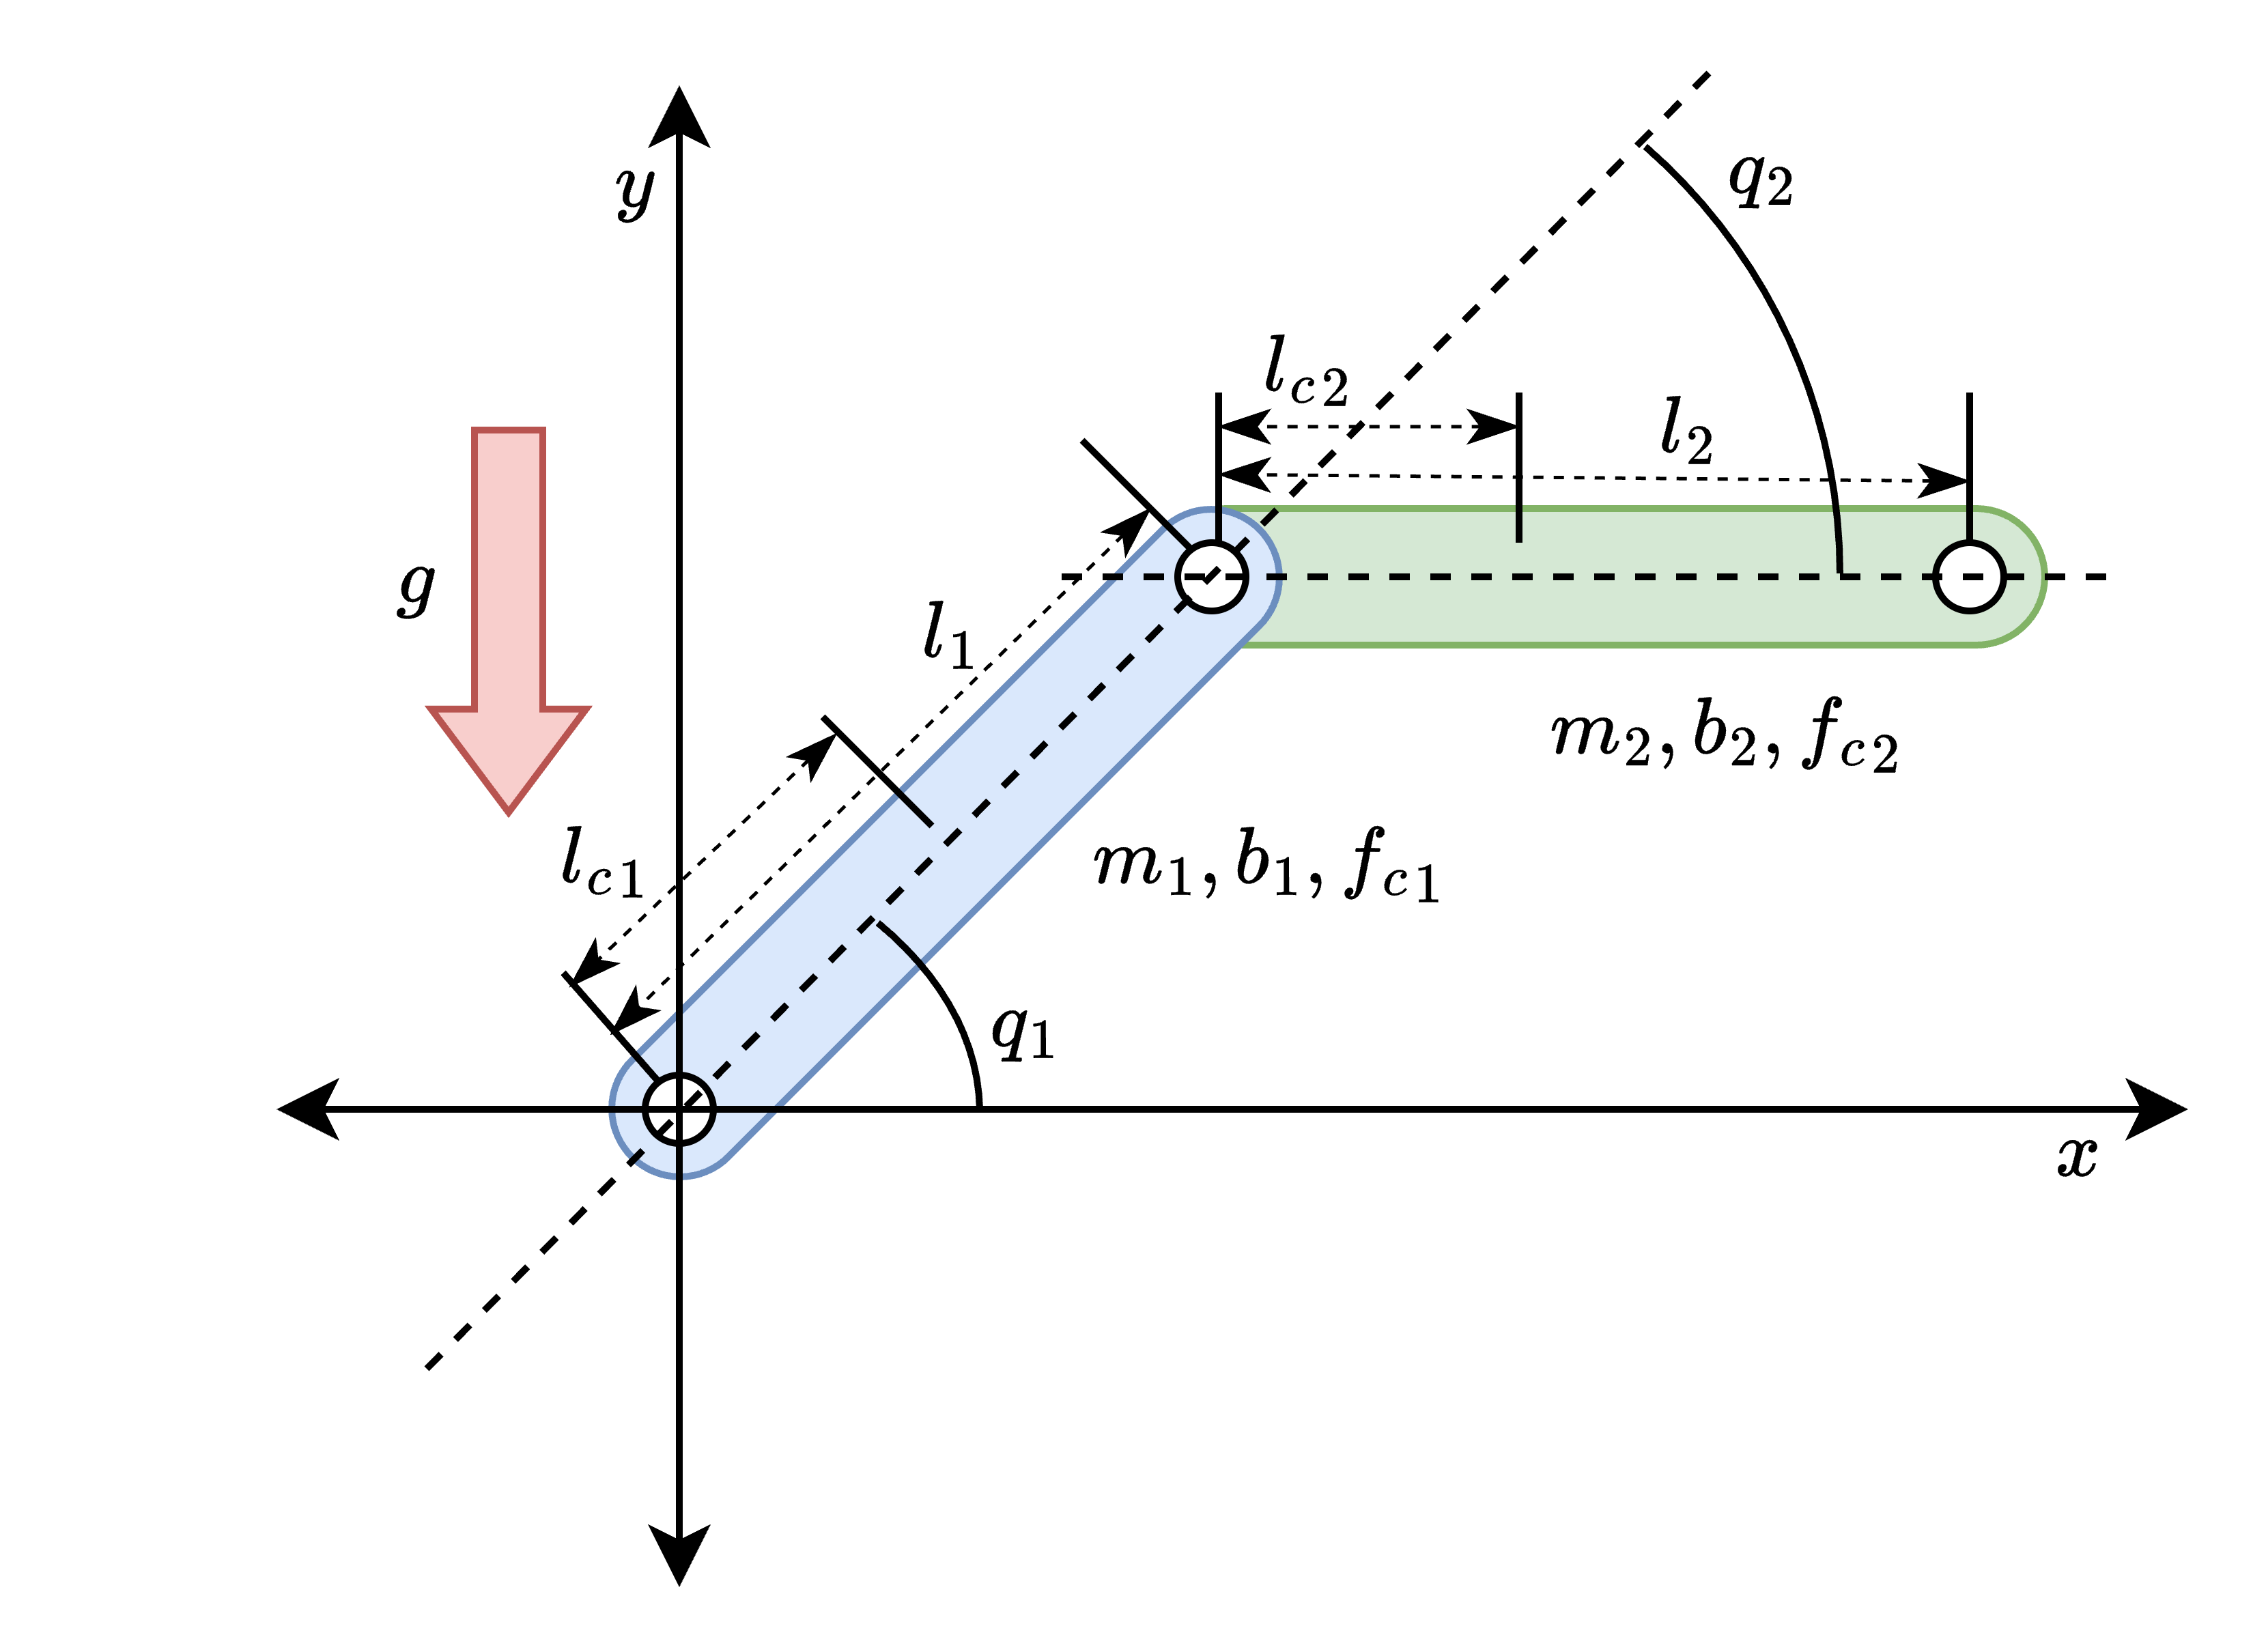
\includegraphics[width=0.8\linewidth]{RobotModel.drawio.png}
    \caption{Two-link manipulator model.}
    \label{fig: manipulator}
\end{figure}

\begin{table}[!t]
    \renewcommand{\arraystretch}{1.3}
    \caption{System model parameters.}
    \centering
    \begin{tabular}{|c||c|c|c|c|}
    \hline
    Symbol & \textbf{Description} & \textbf{Link 1} & \textbf{Link 2} \\
    \hline 
    $m_1, m_2$ & Mass of link    & 23.902 (kg) & 3.88 (kg) \\
    \hline
    $l_1, l_2$  & Length of link   & 0.45 (m) & 0.45 (m) \\
    \hline
    $l_{c1}, l_{c2}$ & COM of link  & 0.091 (m) & 0.048 (m) \\
    \hline
    $\theta_1, b_2$   & Viscous coefficient  &  2.288 (Nms) & 0.172 (Nms) \\
    \hline
    $f_{c1}, f_{c2}$  & Friction coefficient &  7.17 (Nm) & 1.734 (Nm) \\
    \hline
    \end{tabular}
    \label{table: system parameters}
\end{table}

The two-link manipulator model in \cite{RN33} is employed for the simulation demonstration as described in Fig.~\ref{fig: manipulator}.
In the system, the parameters $q_p,{q_d}_p,\tau_p,m_p,l_p,{l_c}_p,b_p$ and ${f_c}_p$ denote the joint angle, desired joint angle, torque, mass, length, center of mass, viscous coefficient, and friction coefficient, respectively, for link $p\in[1,2]$.
The values of the system parameters are given in Table~\ref{table: system parameters}.
The reference signal of $q=[q_1,q_2]^T$ is defined as follows:
\begin{equation*}
    q_d
    =
    \begin{bmatrix}
        {q_d}_1\\
        {q_d}_2
    \end{bmatrix}
    = 
    \begin{bmatrix}
        +\cos(\pi/2 t) + 1 \\
        -\cos(\pi/2 t) - 1 
    \end{bmatrix}
    .
\end{equation*}

For the comparative study, three controllers were selected: the neuro–adaptive controller with $L_2$-regularization (NAC-L2) and with $\epsilon$-modification (NAC-eMod) and the proposed controller with constrained optimization (NAC-CO).
%%%%%%%%%%%%%%%%%%%%%
The performances of the selected controllers are compared based on the tracking performances and the dependencies of the parameters $\lambda$, $\rho$, and $\beta_j$ of NAC-L2, NAC-eMod, and NAC-CO, respectively.
The square root of the integrated squared error (ISE) (i.e., $\sqrt{\int_0^T\Vert\xi\Vert^2\,dt}$, where $T$ denotes a simulation termination time) is utilized to evaluate the tracking performance.
The parameter dependencies of the controllers were examined via various values of the parameters. 
The values ranged from $0.001$ to $1$ across $10$ samples.
%%%%%%%%%%%%%%%%%%%%%

The control laws of all three controllers were the same as those defined in \eqref{eq. control law}.
The adaptation law of NAC-L2 is derived by adding the squared weight term $(1/2)\lambda\hat\theta^T\hat\theta$ to the objective function such that $J_{L_2} = J+(1/2)\lambda\hat\theta^T\hat\theta$, where $\lambda\in\mathbb R_{>0}$ denotes the $L_2$ coefficient.
The adaptation law obtained via the gradient descent method is subsequently adjusted by adding a stabilizing term $-\alpha\lambda\hat\theta$ as follows:
\begin{equation*} 
    \dot{\hat\theta} = 
    {\partial J_{L_2}\over\partial \hat\theta}
    =-\alpha
    \bigg(
        {\partial J\over\partial \hat\theta}+\lambda\hat\theta
    \bigg)
    .
    \label{eq. adap L2}
\end{equation*}
Note that this adaptation law derived based on $L_2$-regularization method in deep learning is inherently the same as the $\sigma$-modification in adaptive control theory, which adds the term $-\alpha\sigma\hat\theta$, where $\sigma\in\mathbb R_{>0}$.
For NAC-eMod, similar to the $\sigma$-modification, the stabilizing function $-\alpha\rho\Vert \tilde z \Vert\hat\theta$ is added to the adaptation law as follows:
\begin{equation*}
    \dot{\hat\theta} = -\alpha
    \bigg(
        {\partial J\over\partial \hat\theta}+\rho\Vert\tilde z\Vert\hat\theta
    \bigg)
    \label{eq. adap eMod}
\end{equation*}
where $\rho\in\mathbb R_{>0}$ denotes the $\epsilon$-modification coefficient.
By $\Vert\tilde z\Vert$, the stabilizing function proportionally increases as the tracking error $\tilde z$ increases.
Therefore, the adaptation attempts to reduce the tracking error mainly without the effect of the stabilizing function if the tracking error is sufficiently regulated.
The adaptation law of NAC-CO is presented in \eqref{eq. adaptation law th}, \eqref{eq. adaptation law L}, and \eqref{eq. adaptation law L max}.
Owing to the stabilizing functions, the weights of NAC-L2 and NAC-eMod are biased since the stabilizing functions drive the weights toward the origin.

All controllers had the same control parameters except their crucial parameters (i.e., $\lambda$, $\rho$ and $\beta_j$) as $k_q=1.1$, $k_z=10$, $M_0=I_2$ and $W=\text{diag}([5,1,15,15])$.
The parameters of the NNs were set to $l_0=2$, $l_1=16$, $l_2=2$, and $\alpha=10^3$, and the same random seed was applied for weight initialization.
The NN input vector was set to the desired trajectory $q_d$, with the augmented 1 to incorporate the bias term in the weight matrix such that $q_{NN}=[q_d^T,1]^T$.
For NAC-CO, the parameters of the weight norm constraints were set as $\bar\theta_0=10$ and $\bar\theta_1=20$.
The sampling time of the simulation and the simulation termination time were set to $T_s=10^{-4}$ and $T=10$, respectively.

\subsection{Results}

\begin{figure}[!t]      
    \centering
    {\includegraphics[width=.85\linewidth]{BoxWhisker.drawio.png}}
\caption{Box-and-Whisker plot of the square root of the tracking ISEs of NAC-L2, NAC-eMod and NAC-CO across various parameter values.}
    \label{fig: Box-beard plot}
\end{figure}

\begin{table}[!t]
    \renewcommand{\arraystretch}{1.3}
    \caption{Quantitative comparison of square root of tracking ISE.}
    \centering
    \begin{tabular}{|c||c|c|c|}
    \hline
     & \textbf{NAC-L2} & \textbf{NAC-eMod} & \textbf{NAC-CO} (proposed) 
     \\
    \hline 
    Maximum         & $11.1753$e-3 & $0.5603$e-3 & $0.3439$e-3 \\
    \hline
    % Upper quartile  & $1.7284$e-3 & $0.5566$e-3 & $0.3261$e-3 \\
    % \hline
    Median          & $0.5898$e-3 & $0.5519$e-3 & $0.3240$e-3 \\
    \hline
    % Lower quartile  & $0.5533$e-3 & $0.5470$e-3 & $0.3238$e-3 \\
    % \hline
    Minimum         & $0.5434$e-3 & $0.5434$e-3 & $0.3235$e-3 \\
    \hline
    \end{tabular}
    \label{table: error norm}
\end{table}

As shown in Fig.~\ref{fig: Box-beard plot}, the maximum square root of the tracking ISE of NAC-CO is smaller than the minimum square root of the tracking ISEs of NAC-L2 and NAC-eMod for all variations in the parameters.
This is because NAC-L2 and NAC-eMod bias the weights to the origin due to the presence of stabilizing functions.
A quantitative comparison of the square root of the tracking ISE is provided in Table~\ref{table: error norm}.

\begin{figure}[!t]      
    \centering
        \subfloat[NAC-L2]{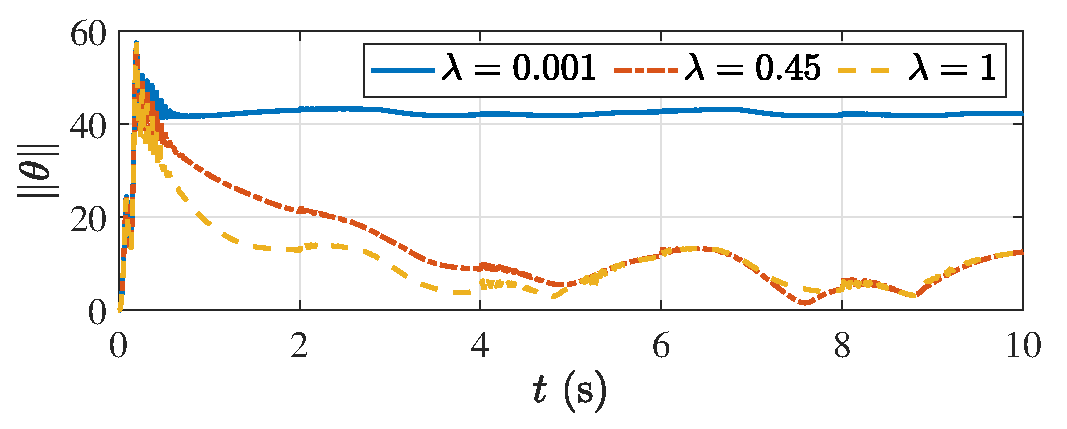
\includegraphics[width=.85\linewidth]{fig9.eps}%
        \label{fig: weight NAC-L2}}
    \vfill
        \subfloat[NAC-eMod]{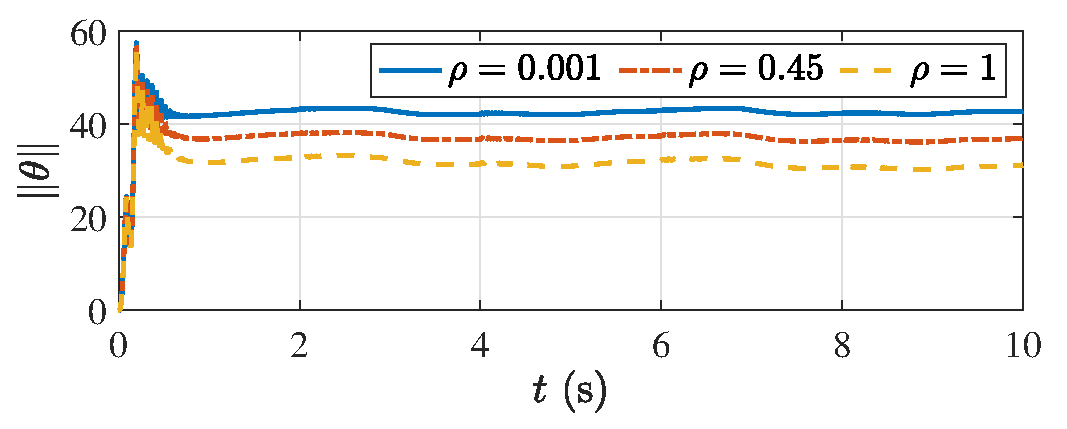
\includegraphics[width=.85\linewidth]{fig10.eps}%
        \label{fig: weight NAC-eMod}}
    \vfill
        \subfloat[NAC-CO]{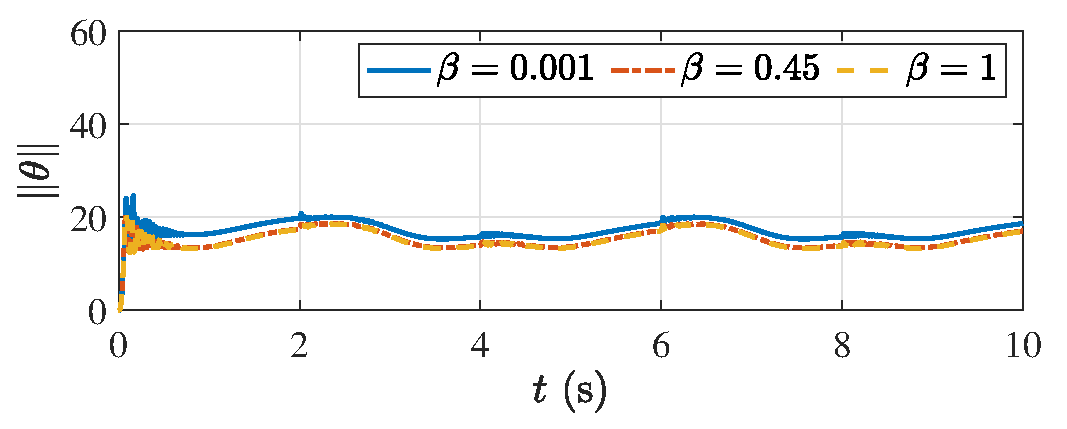
\includegraphics[width=.85\linewidth]{fig8.eps}%
        \label{fig: weight NAC-CO}}
    \vfill
    \caption{Weight norms of NAC-L2, NAC-eMod, and NAC-CO.}
    \label{fig: weight}
\end{figure}

\begin{figure}[!t]      
    \centering
        \subfloat[NAC-L2]{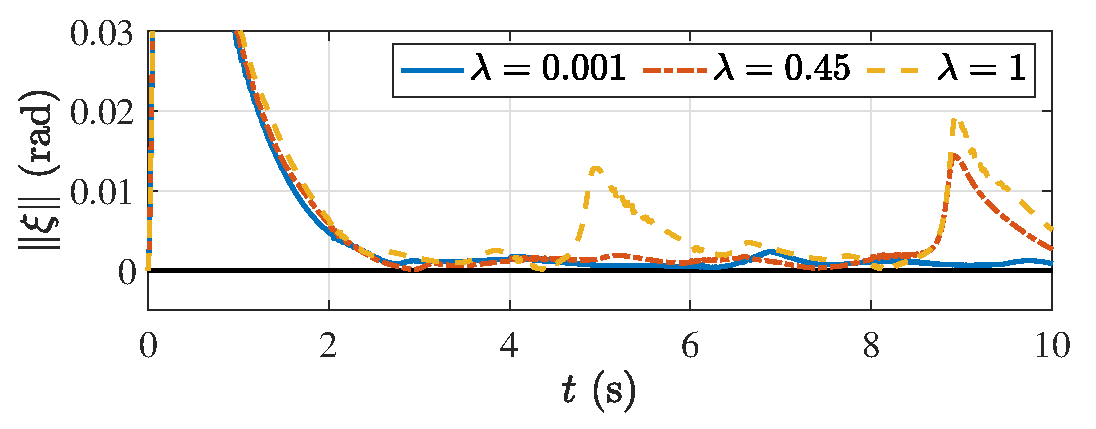
\includegraphics[width=.85\linewidth]{fig6.eps}%
        \label{fig: error NAC-L2}}
    \vfill
        \subfloat[NAC-eMod]{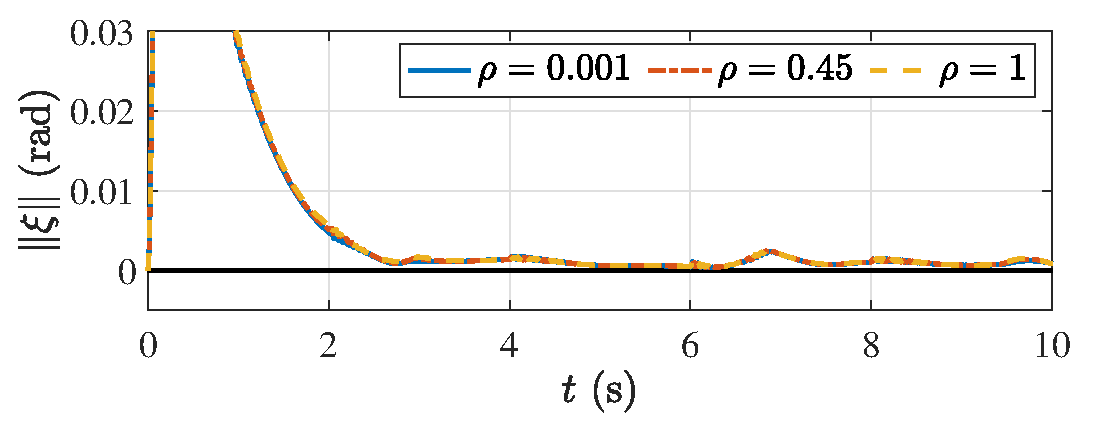
\includegraphics[width=.85\linewidth]{fig7.eps}%
        \label{fig: error NAC-eMod}}
    \vfill
        \subfloat[NAC-CO]{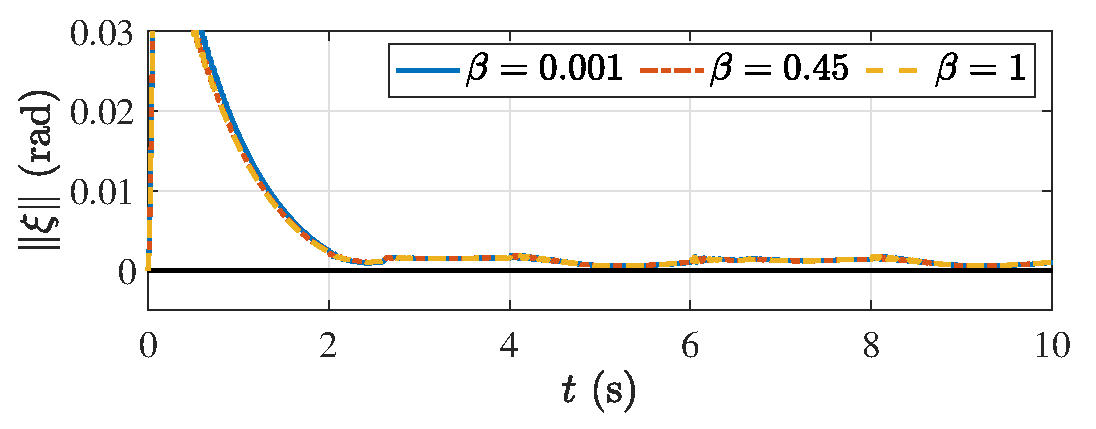
\includegraphics[width=.85\linewidth]{fig5.eps}%
        \label{fig: error NAC-CO}}
    \vfill
    \caption{Tracking errors of NAC-L2, NAC-eMod, and NAC-CO.}
    \label{fig: error}
\end{figure}

For the detailed analysis, three values of the parameters (i.e., $\lambda,\rho,\beta_j\in[0.001,0.45,1]$) were selected as described in Fig.~\ref{fig: weight} and Fig.~\ref{fig: error}.
As shown in Fig.~\ref{fig: weight NAC-L2}, increasing $\lambda$ reduces the weight norm of NAC-L2 via the stabilizing function $-\alpha\lambda\hat\theta$.
Moreover, the high dependency of NAC-L2 on the $L_2$-regularization coefficient $\lambda$ can also be observed.
Since the weight norm is decreased, NAC-L2 cannot generate sufficient control inputs, resulting in a larger square root of tracking ISE, as shown in Fig.~\ref{fig: error NAC-L2}.

On the other hand, NAC-eMod has a lower dependency on the $\epsilon$-modification coefficient $\rho$, as shown in Fig.~\ref{fig: weight NAC-eMod} and Fig.~\ref{fig: error NAC-eMod}.
This is because the stabilizing function $-\alpha\rho\Vert\tilde z\Vert\hat\theta$ can be decreased once the tracking error $\tilde z$ is sufficiently regulated.
However, the bias of the weights to the origin still exists, as described in Fig.~\ref{fig: weight NAC-eMod} (i.e., smaller weight norms are observed as $\rho$ increases. ).
Therefore, similar to NAC-L2, the biased weights produce insufficient control input, resulting in a relatively larger square root of tracking ISE than that of NAC-CO, as described in Table \ref{table: error norm}.

Finally, the weight norm of NAC-CO is smaller than those of NAC-L2 and NAC-eMod, as shown in Fig.~\ref{fig: weight NAC-CO}, with better tracking performance.
Even if a large $\beta_j$ is provided, NAC-CO can adjust the adaptation direction to satisfy the weight norm constraints faster, according to \eqref{eq. adaptation law L}.
Therefore, the lowest dependency on the update rate $\beta_j$ is observed in NAC-CO, as shown in Fig.~\ref{fig: weight NAC-CO} and Fig.~\ref{fig: error NAC-CO}.
Note that $\beta_j$ of NAC-CO is the update rate for the Lagrange multipliers, whereas $\lambda$ and $\rho$ are the coefficients of the stabilizing function that generates the biases of the weights.
However, considering the implementation using a digital computer, excessively large $\beta_j$ values should be avoided.

The details of the satisfaction of the weight norm constraints are shown in Fig.~\ref{fig: weight and multiplier} for NAC-CO with $\beta_j=0.001$.
As the weight norms of each layer reach the constraint boundary, the corresponding Lagrange multipliers are generated.
Using the Lagrange multipliers, the adaptation direction is adjusted toward the constraint satisfactory point.
The Lagrange multipliers disappear when the constraints are satisfied, and the weights are adapted to optimize the original objective function without weight bias.

\begin{figure}[!t]      
    \centering
    \subfloat[Weight norm]{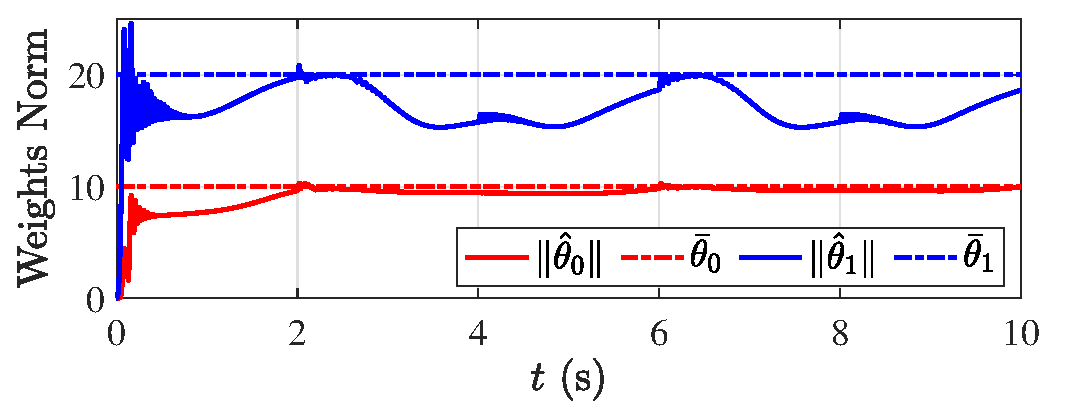
\includegraphics[width=.8 \linewidth]{fig12.eps}%
    \label{fig: weight per layer NAC-CO}}
    \vfill
    \subfloat[Lagrange multipliers]{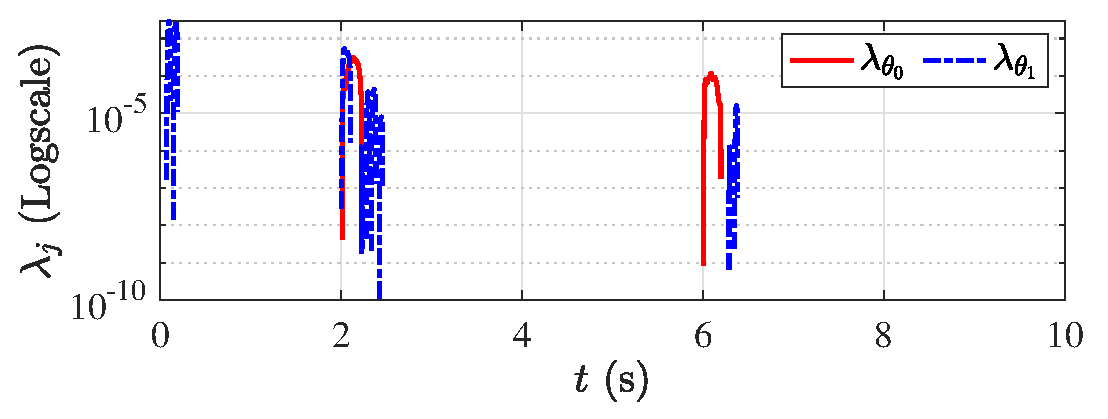
\includegraphics[width=.8 \linewidth]{fig11.eps}%
    \label{fig: multipliers NAC-CO}}
    \caption{Weight norms and Lagrange multipliers of NAC-CO ($\beta=0.001$).}
    \label{fig: weight and multiplier}
\end{figure}

Furthermore, it is important to note that NAC-CO shows enhanced tracking performance with smaller weights than NAC-L2 and NAC-eMod.
This implies that the weights in NAC-CO approach the different local optimal solution points from those of NAC-L2 and NAC-eMod.
Therefore, if the physical analysis of the system is available to predict the feasible maximum control inputs, NAC-CO can find the local optimal solution without unnecessarily large control inputs by imposing proper weight norm constraints.


%  SECTION CONCLUSION ======================================
\section{Conclusion}\label{sec:conclusion}

\color{black}
In this paper, a neuro–adaptive control method is proposed for uncertain Euler‒Lagrange systems, ensuring weight boundedness.
Adaptation laws are derived by formulating a constrained optimization problem with weight norm constraints.
The boundedness of the tracking error and the weight estimation are analyzed via Lyapunov analysis.
The simulation results demonstrate that the proposed controller outperforms the existing methods in terms of tracking performance and parameter dependency.
As further work, the state and output constraints for safety will be handled, ensuring stability.
\color{black}

\addtolength{\textheight}{-12cm}   % This command serves to balance the column lengths
                                  % on the last page of the document manually. It shortens
                                  % the textheight of the last page by a suitable amount.
                                  % This command does not take effect until the next page
                                  % so it should come on the page before the last. Make
                                  % sure that you do not shorten the textheight too much.

%%%%%%%%%%%%%%%%%%%%%%%%%%%%%%%%%%%%%%%%%%%%%%%%%%%%%%%%%%%%%%%%%%%%%%%%%%%%%%%%



%%%%%%%%%%%%%%%%%%%%%%%%%%%%%%%%%%%%%%%%%%%%%%%%%%%%%%%%%%%%%%%%%%%%%%%%%%%%%%%%



%%%%%%%%%%%%%%%%%%%%%%%%%%%%%%%%%%%%%%%%%%%%%%%%%%%%%%%%%%%%%%%%%%%%%%%%%%%%%%%%
% \section*{APPENDIX}

% Appendixes should appear before the acknowledgment.

% \section*{ACKNOWLEDGMENT}

% The preferred spelling of the word ÒacknowledgmentÓ in America is without an ÒeÓ after the ÒgÓ. Avoid the stilted expression, ÒOne of us (R. B. G.) thanks . . .Ó  Instead, try ÒR. B. G. thanksÓ. Put sponsor acknowledgments in the unnumbered footnote on the first page.



%%%%%%%%%%%%%%%%%%%%%%%%%%%%%%%%%%%%%%%%%%%%%%%%%%%%%%%%%%%%%%%%%%%%%%%%%%%%%%%%

\bibliographystyle{ieeetr}
\bibliography{refs}

\end{document}


% \begin{figure}[!t]
%     \centering
%         \subfloat[ of Proposed]{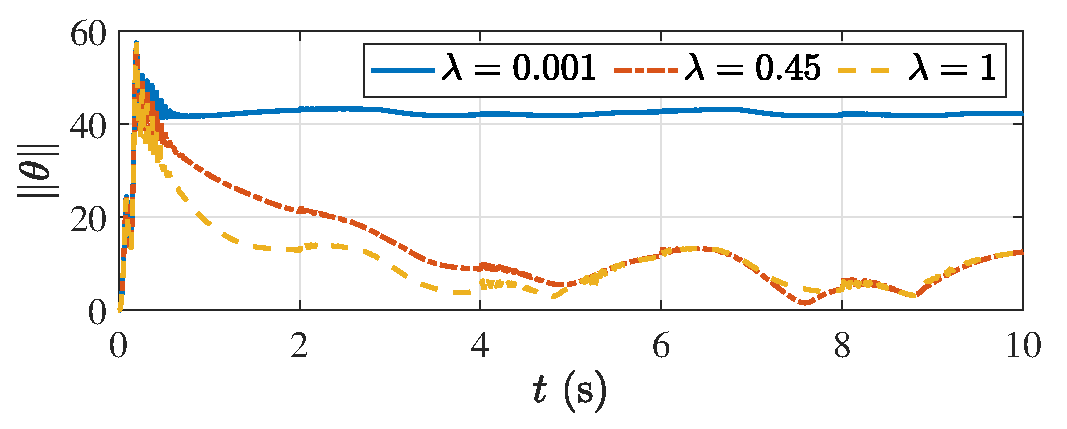
\includegraphics[width=0.45\linewidth]{fig9.eps}%
%         \label{fig: weight_Proposed}}
%     \qquad
%         \subfloat[ of NAC-L2]{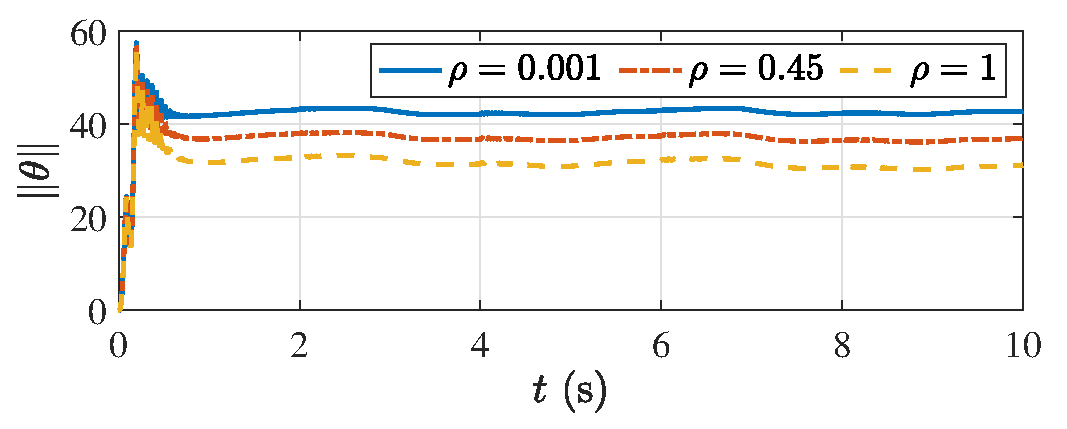
\includegraphics[width=0.45\linewidth]{fig10.eps}%
%         \label{fig: weight_NAC-L2}}
%     \vfill
%         \subfloat[ of NAC-eMod]{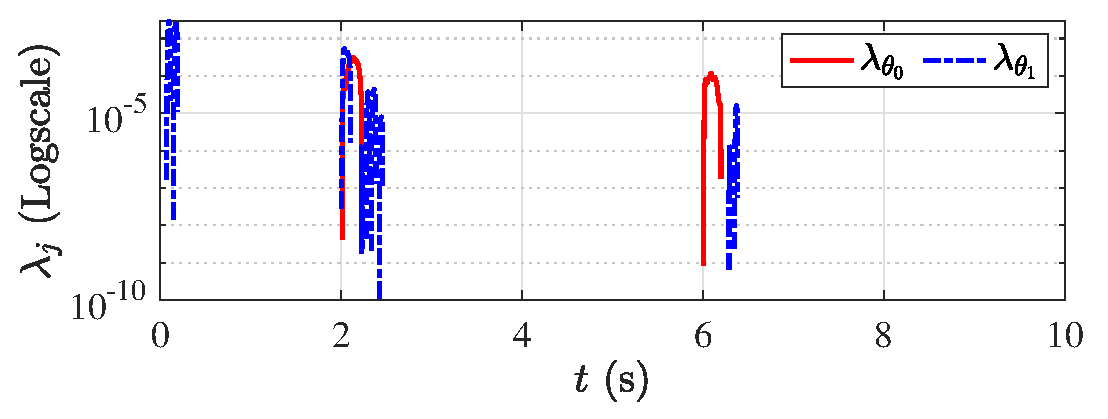
\includegraphics[width=0.45\linewidth]{fig11.eps}%
%         \label{fig: weight_NAC-eMod}}
%     \qquad
%         \subfloat[ of CM3]{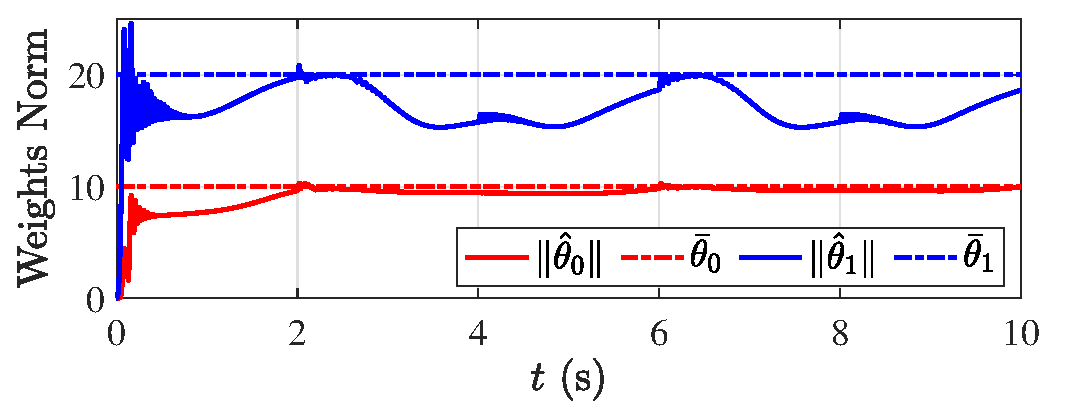
\includegraphics[width=0.45\linewidth]{fig12.eps}%
%         \label{fig: weight_CM3}}
%     \caption{controls.}
%     \label{fig: weights}
% \end{figure}
